% !TEX root = ejemplo.tex

\chapter{Tikz}
Tikz es un paquete muy amplio y es bastante difícil describir todas sus
capacidades. Por ejemplo el manual, que hace precisamente eso, es de mas de
\num{1000} páginas. Por esta razón sólo veremos lo más básico de este paquete. Además, un buen sitio para aprender más de lo que viene aquí es \url{https://latexdraw.com}.

\section{Nodos y líneas}%
\label{sec:basic}
Tikz crea un plano cartesiano en la página. Así para poner contenido se
específica una coordenada o bien una recta entre dos puntos del plano, como
en el siguiente ejemplo.
\begin{center}
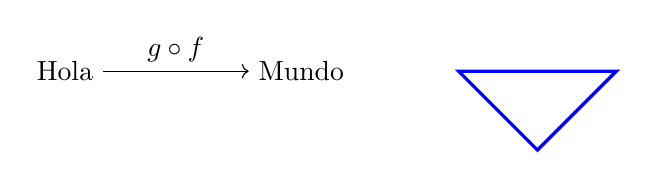
\begin{tikzpicture}
\node (x) at (0,0) {Hola};
\node (y) at (3,0) {Mundo};
\draw[->] (x) --node[above] {\(g\circ f\)} (y);
\draw[blue, very thick] (5,0) -- (7,0) -- (6,-1) -- cycle;
\end{tikzpicture}
\end{center}
La sintaxis \verb|\node (x) at (0,0) {Hola};| crea un nodo con el contenido
\enquote{Hola} en la posición \((0,0)\) y le pone una etiqueta \enquote{(x)} para futuras
referencias. En la flecha de (x) a (y) se puso un nodo sobre la flecha con
el comando \verb|\draw[->] (x) --node[above] {\(g\circ f\)} (y);|. Las
opciones de posición son \texttt{above}, \texttt{below}, \texttt{left} y
\texttt{right}. Para mover de posición el nodo se puede usar \texttt{near
start}, \texttt{near end}, \texttt{center} (la opción por defecto) o una más
granular \texttt{pos=x}, donde \texttt{x} es un número entre 0 y 1.

Algunas figuras ya están definidas en la base de tikz. Algunas de ellas son:
\begin{center}
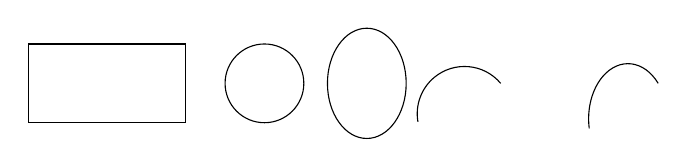
\begin{tikzpicture}
\draw (0,-0.5) rectangle (2,0.5);
\draw (3,0) circle [radius=5mm];
\draw (4.3,0) ellipse [x radius=5mm, y radius=7mm];
\draw (6,0) arc [start angle= 40, end angle=190, radius=6mm];
\draw (8,0) arc [start angle= 40, end angle=190, x radius=5mm, y radius=7mm];
\end{tikzpicture}
\end{center}
Hay muchas más en la librería \texttt{shapes} o \texttt{shapes.geometric}.

También se pueden hacer curvas \enquote{jalando} una línea en dos puntos
\begin{center}
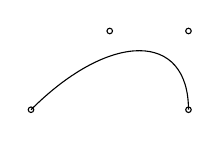
\begin{tikzpicture}
\draw (0,0) circle (1pt); % nodo de referencia
\draw (1,1) circle (1pt); % nodo de referencia
\draw (2,1) circle (1pt); % nodo de referencia
\draw (2,0) circle (1pt); % nodo de referencia
\draw (0,0) .. controls (1,1) and (2,1) .. (2,0);
\end{tikzpicture}
\end{center}
donde los puntos de arriba sólo fueron puestos para hacer referencia de qué
puntos se \enquote{jalo} la recta.

Colorear figuras también es fácil, además de que se pueden hacer muchos
estilos de coloreado.
\begin{center}

\begin{tikzpicture}
\fill[blue!50,rounded corners] (0,0) rectangle (1,1);
\filldraw[fill=red!30, draw=red] (2,.5) circle (3mm);
\shade[left color=red, right color=blue] (3,0) rectangle (5,1);
\shade[inner color=red, outer color=blue] (6,0) rectangle (8,1);
\shade[ball color=violet!50] (9.5,.5) circle (5mm);
\fill[blue!50,rounded corners,opacity=0.5] (11,0) rectangle (12,1);
\end{tikzpicture}
\end{center}

Una aplicación de la opción \texttt{opacity} es hacer diagramas de Venn. Para
esto voy a usar coordenadas polares. Estas usan la sintaxis
(ángulo:longitud).
\begin{center}
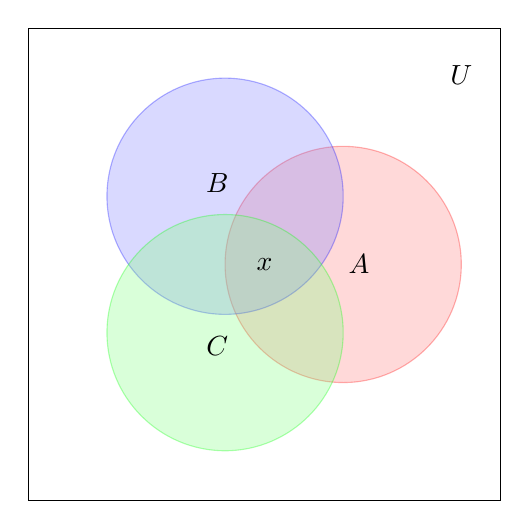
\begin{tikzpicture}
\filldraw[fill=red!50,draw=red,opacity=0.3] (0:1cm) circle (1.5cm);
\filldraw[fill=blue!50,draw=blue,opacity=0.3] (120:1cm) circle (1.5cm);
\filldraw[fill=green!50,draw=green,opacity=0.3] (240:1cm) circle (1.5cm);
\node at (0:0) {\(x\)};
\node at (0:1.2cm) {\(A\)};
\node at (120:1.2cm) {\(B\)};
\node at (240:1.2cm) {\(C\)};
\draw (-3,-3) rectangle (3,3);
\node at (2.5,2.4) {\(U\)};
\end{tikzpicture}
\end{center}

Una aplicación de \texttt{arc} puede ser dibujar un cilindro
\begin{center}
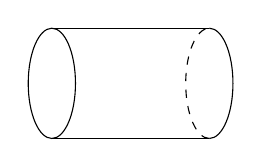
\begin{tikzpicture}[x=1mm, y=1mm]
\draw (0,0) ellipse [x radius=3mm, y radius=7mm];
\draw[dashed] (20,-7) arc [start angle=270,end angle=90,x radius=3mm,y radius=7mm];
\draw[rotate around={180:(20,0)}] (20,7) arc [start angle=90,end angle=270,x radius=3mm,y radius=7mm];
\draw (0,7) -- (20,7) (0,-7) -- (20,-7);
\end{tikzpicture}
\end{center}

A pesar de que esto es lo más básico de Tikz se pueden tener muchas
posibilidades combinando estas reglas básicas entre ellas.

Otra función de Tikz es graficar funciones. En el siguiente ejemplo
graficamos una parábola y el seno. En las funciones trigonométricas se debe
especificar como se hacen los cálculos: radianes, grados, etc. Para obtener
el seno como queremos se escribe \verb|sin((\y)r)|.
\begin{center}
\begin{tikzpicture}
\draw[->] (-3,0) -- (3,0)node[right] {\(x\)};
\draw[->] (0,-1) -- (0,4)node[above] {\(y\)};
\draw[domain=-2:2, variable=\x] plot ({\x},{\x * \x});
\draw[domain=-4:4,variable=\y,blue,smooth] plot ({\y},{sin((\y)r)});
\end{tikzpicture}
\end{center}
Esta forma simple es bastante efectiva y su única posible desventaja es que
se debe tener cuidado con las dimensiones de la gráfica para que no haya
algunas muy grandes y otras muy chicas, generando una inconsistencia
indeseada.

Tikz es la capa superior de \texttt{pgf} así los métodos de Tikz serán muy
similares a los de \texttt{pgf}. Por esta razón otro método para graficar es
usar el paquete \texttt{pgfplots} que usará el motor de \texttt{pgf} para
hacer gráficas. Es importante notar que se escribió
\verb|\pgfplotsset{width=6cm,compat=1.17}| en el preámbulo. La parte de
\texttt{width} es para que todas las gráficas tengan el mismo tamaño y así
tener uniformidad en el texto. La parte de \texttt{compat} es la versión del
motor que se usará, diferentes versiones podrían generar diferentes salidas
con el mismo código. Para usar la versión más actual siempre se escribe
\texttt{compat=newest}, aunque esta opción no es recomendada ya que es como
trabajar con una versión beta de pgf y como se mencionó antes la salida del
mismo código podría cambiar.
\begin{center}
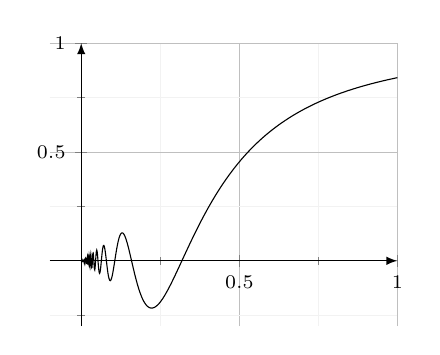
\begin{tikzpicture}
\begin{axis}[
    xmin=-0.1,xmax=1,
    ymin=-0.3,ymax=1,
    grid=both,
    grid style={line width=.1pt, draw=gray!10},
    major grid style={line width=.2pt,draw=gray!50},
    axis lines=middle,
    minor tick num=1,
    axis line style={-latex},
    ticklabel style={font=\scriptsize}
]
  \addplot [domain=-0.001:1,samples=800,smooth] {x*sin((1/x)r)};
  %\addlegendentry{nombre de la función}
  \end{axis}
\end{tikzpicture}
\end{center}


\section{Diagramas conmutativos}
Una aplicación que seguramente tendrá mayor uso en la carrera de matemáticas
es dibujar diagramas conmutativos. En la sección~\ref{sec:basic} ya hicimos
una flecha entre dos objetos con un nombre sobre dicha flecha. Con la misma
técnica se pueden hacer diagramas conmutativos. Aquí veremos como se
hacen usando \verb|\usetikzlibrary{cd}| o equivalentemente
\verb|\usepackage{tikz-cd}|.
\begin{center}
\begin{tikzcd}
T\ar[bend left=30]{rrd}{h_{1}}\ar[bend right=30]{rdd}[swap]{h_{2}}\ar[dashed]{rd}[description]{h}\\[-3mm]
&[-2mm] P\ar{r}{p_{1}}\ar{d}{p_{2}} & A\ar{d}{f}\\
& B\ar{r}[swap]{g} & C
\end{tikzcd}
\end{center}

Esta forma de hacer diagramas por medio de matrices podría parecer limitada
respecto a la de coordenadas con \texttt{tikzpicture}, pero los métodos de
tikz son suficientemente robustos como para hacer el siguiente diagrama con
matrices (este usa la librería \texttt{calc} para mover fácilmente la flecha
\(\bar{\eta}\)):
\begin{center}
\begin{tikzcd}[
 execute at end picture={
   \draw [/tikz/commutative diagrams/double line,-Implies] ($(f1)+(5mm,5mm)$) --node[right]{$\bar{\eta}$} ($(f1)+(5mm,-5mm)$);
 }
]%para que la \eta del final salga donde quiero
%primer renglón
&&&&&&&[-5mm]&[-5mm]
\mathcal{F} \\[-15pt]
% segundo renglón
&&&&&
\mathcal{F}
\ar[bend left=5]{rrru}{1_{\mathcal{F}}}
\ar{rd}[name=g1]{g_{*}}
\ar[bend left=45]{rrdd}[name=f1]{f_{*}}
&&&  \\[-5pt]
%tercer renglón
&&&&
|[alias=e1]|\mathcal{E}
\ar{ur}{g^{*}}
\ar{drrr}[swap,name=p1]{p_{*}}
&&
\mathcal{E}
\ar{dr}[swap]{p_{*}}
&&  \\[-5pt]
%cuarto renglón
\mathcal{E}
\ar{rr}[name=1e]{1_{\mathcal{E}}}
\ar{dr}[swap]{g{*}}
&&
\mathcal{E}
\ar{r}{p_{*}}
&
|[alias=s1]|\mathcal{S}
\ar{ur}{p^{!}}
\ar[bend right=5]{rrrr}[swap, name=1s]{1_{\mathcal{S}}}
&&&&
\mathcal{S}
\ar[bend right=10]{ruuu}[swap]{f^!}
&  \\[-5pt]
%quinto renglón
&
|[alias=f2]|\mathcal{F}
\ar{ur}[swap]{g_{*}}
\ar[bend right=15]{urr}[swap]{f_{*}}
&&&&&&&
%transformaciones naturales
\arrow[Rightarrow,from=g1, to=p1,shorten >=3mm,shorten <=3mm]{}[swap]{(p_{*}\nu)^{-1}}
\arrow[Rightarrow,from=1e, to=f2,shorten >=1mm,shorten <=2mm]{}[swap]{\nu}
\arrow[Rightarrow,from=e1, to=1s,shorten >=3mm,shorten <=2mm]{}[swap]{\varepsilon}
\end{tikzcd}
\end{center}

Hay otros paquetes para hacer diagramas conmutativos, uno que aún es muy
común es \texttt{xy-pic}. También tiene una versión de su sintaxis similar
a la de \texttt{tikzpicture} de arriba y una versión de matriz como la de
\texttt{tikzcd}. A pesar de ser común en estos días creo que el paquete que
debería usarse es \texttt{tikz} ya que \texttt{xy-pic} tiene cosas que
están mal medidas y tiene muchos años que no tiene mantenimiento. Tiene
tantos años sin mantenimiento que se quedo sin soportar la compilación con
Lua\LaTeX, por lo que no es posible mostrar un ejemplo con este método de
compilación. En la compilación con pdf\LaTeX{} se puede ver que al dibujar
un monomorfismo o una inclusión, las flechas quedan demasiado cerca del
dominio.
\ifpdftex
\begin{minipage}{0.45\linewidth}
\centering
Con \texttt{xy-pic}
  \[
  \begin{xy}
    (0,0) *+{C} = "c1",
    (0,-10) *+{D} = "d1",
    (10,0) *+{C} = "c2",
    (10,-10) *+{D} = "d2",
    \POS "c1" \ar@{>->} "d1",
    \POS "c2" \ar@{^{(}->} "d2",
  \end{xy}
  \]
\end{minipage}%
\begin{minipage}{0.45\linewidth}
\centering
Con \texttt{tikz-cd}
  \begin{center}
    \begin{tikzcd}
      C\ar[tail]{d} & C\ar[hook]{d}\\
        D & D
    \end{tikzcd}
    \end{center}
\end{minipage}
\fi


\section{Visualización de datos}
No he tenido la necesidad de trabajar visualizando información de una base
de datos, así que no tengo un ejemplo útil de esto. Sin embargo, en el
manual de tikz/pgf el capítulo 80 se encarga de esto. Afortunadamente este
es un manual muy bien escrito y con muchos ejemplos, así que una mirada
rápida dará los conceptos básicos para hacer conjuntos de datos dentro del
documento o usar conjuntos de datos de un archivo \texttt{.csv},
\texttt{.dat},\ldots

Aún así va un intento de ejemplos. Para esto voy a usar las librerías
\texttt{datavisualization} y \texttt{datavisualization.formats.functions}. Un ejemplo del manual:
\begin{center}
\begin{tikzpicture}
\datavisualization [school book axes, visualize as smooth line]
  data {
    x, y
    -1.5, 2.25
    -1, 1
    -.5, .25
    0, 0
    .5, .25
    1, 1
    1.5, 2.25
  };
\end{tikzpicture}
\end{center}


\section{Por diversión, Fractales}
Con \verb|\usetikzlibrary{decorations.fractals}|
\begin{center}
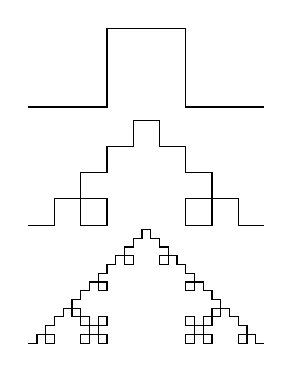
\begin{tikzpicture}[decoration=Koch curve type 1]
\draw decorate{ (0,0) -- (3,0) };
\draw decorate{ decorate{ (0,-1.5) -- (3,-1.5) } };
\draw decorate{ decorate{ decorate{ (0,-3) -- (3,-3) } } };
\end{tikzpicture}
\qquad\qquad
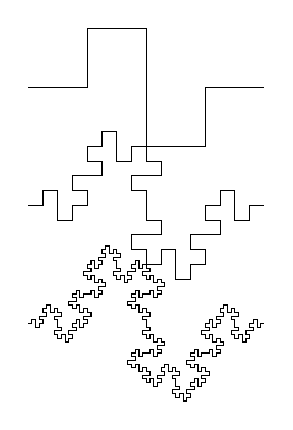
\begin{tikzpicture}[decoration=Koch curve type 2]
\draw decorate{ (0,0) -- (3,0) };
\draw decorate{ decorate{ (0,-1.5) -- (3,-1.5) } };
\draw decorate{ decorate{ decorate{ (0,-3) -- (3,-3) } } };
\end{tikzpicture}
\qquad\qquad
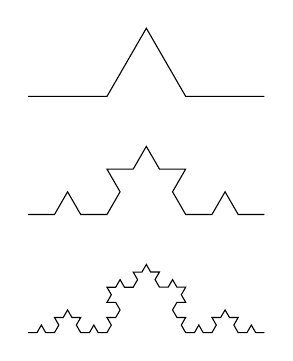
\begin{tikzpicture}[decoration=Koch snowflake]
\draw decorate{ (0,0) -- (3,0) };
\draw decorate{ decorate{ (0,-1.5) -- (3,-1.5) } };
\draw decorate{ decorate{ decorate{ (0,-3) -- (3,-3) } } };
\end{tikzpicture}
\vspace{1em}
\begin{tikzpicture}[decoration=Cantor set]
\draw decorate{ (0,0) -- (3,0) };
\draw decorate{ decorate{ (0,-.5) -- (3,-.5) } };
\draw decorate{ decorate{ decorate{ (0,-1) -- (3,-1) } } };
\end{tikzpicture}
\end{center}

Con \verb|\usetikzlibrary{shadings}| tenemos un Mandelbrot, si hacen esto en
overleaf hay que cambiar el visor de pdf para que sí aparezca el dibujo.
Esto se hace desde el menú en la parte superior izquierda.
\begin{center}
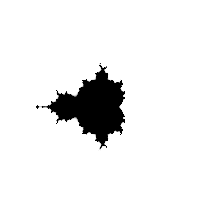
\begin{tikzpicture}
\shade[shading=Mandelbrot set] (0,0) rectangle (2,2);
\end{tikzpicture}
\end{center}

Con \verb|\usetikzlibrary{lindenmayersystems}|
\begin{center}
\begin{tikzpicture}
\pgfdeclarelindenmayersystem{Koch curve}{
\rule{F -> F-F++F-F} }
\shadedraw [top color=white, bottom color=blue!50, draw=blue!50!black] [l-system={Koch curve, step=2pt, angle=60, axiom=F++F++F, order=3}] lindenmayer system -- cycle;
\end{tikzpicture}
\quad
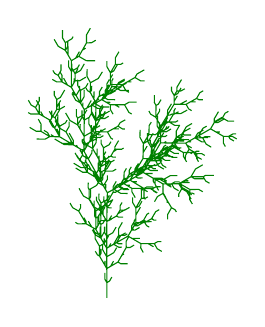
\begin{tikzpicture}
\draw [green!50!black, rotate=90]
[l-system={rule set={F -> FF-[-F+F]+[+F-F]}, axiom=F, order=4, step=2pt, randomize step percent=25, angle=30, randomize angle percent=5}]
  lindenmayer system;
\end{tikzpicture}
\end{center}

Girasol de \url{https://www.texample.net}

\def\nbrcircles {377}
\def\outerradius {30mm}
\def\deviation {.9}
\def\fudge {.62}

\newcounter{cumulArea}
\setcounter{cumulArea}{0}

\begin{center}
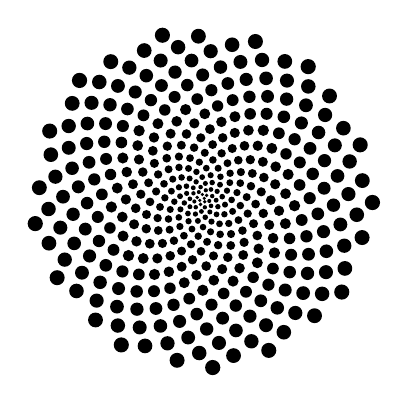
\begin{tikzpicture}[scale=.1]

\pgfmathsetmacro {\goldenRatio} {(1+sqrt(5))}
\pgfmathsetmacro {\meanArea}
      {pow(\outerradius * 10 / \nbrcircles, 2) * pi}
\pgfmathsetmacro {\minArea} {\meanArea * (1 - \deviation)}
\pgfmathsetmacro {\midArea} {\meanArea * (1 + \deviation) - \minArea}

\foreach \b in {0,...,\nbrcircles}{
    % mod() must be used in order to calculate the right angle.
    % otherwise, when \b is greater than 28 the angle is greater
    % than 16384 and an error is raised ('Dimension too large').
    % -- thx Tonio for this one.
    \pgfmathsetmacro{\angle}{mod(\goldenRatio * \b, 2) * 180}

    \pgfmathsetmacro{\sratio}{\b / \nbrcircles}
    \pgfmathsetmacro{\smArea}{\minArea + \sratio * \midArea}
    \pgfmathsetmacro{\smRadius}{sqrt(\smArea / pi) / 2 * \fudge}
    \addtocounter{cumulArea}{\smArea};

    \pgfmathparse{sqrt(\value{cumulArea} / pi) / 2}
    \fill[] (\angle:\pgfmathresult) circle [radius=\smRadius] ;
}
\end{tikzpicture}
\end{center}

Uno más usando la librería \texttt{math}
\begin{center}
\begin{tikzpicture}[line cap=round, x=2cm,y=2cm, line join=round]
\tikzmath{%
  int \n;
  \b = 0; \d = 1;
  for \n in {1,...,10}{
    \l = (\n == 10 && 10 > 1) ? "red" : "black";
    \e = (\n == 1) ? " -- cycle" : "";
    {
      \path [rotate=\b, draw=\l] (0,0) -- (\d,1) -- (\d,0)
        node [\l, midway, anchor=\b+180] {1}
        \e (\d/2, 0)  node [fill=white] {$\sqrt{\n}$};
      \path [draw=\l, rotate=\b] (\d-.1,0) |- ++(.1,.1);
    };
    \d = sqrt(1+(\d)^2); \b = \b + asin(1/\d);
  };
  {
    \path [rotate=\b, \l] (\d/2, 0) node [fill=white] {$\sqrt x$};
  };
}
\end{tikzpicture}
\end{center}
